%	% ****** Start of file MolecularSpinFlipLoss.tex ******
%
%
%

\documentclass[%
 reprint,
%superscriptaddress,
%groupedaddress,
%unsortedaddress,
%runinaddress,
%frontmatterverbose, 
%preprint,
%showpacs,preprintnumbers,
%nofootinbib,
%nobibnotes,
%bibnotes,
 amsmath,amssymb,
 aps,
prl,
%pra,
%prb,
%rmp,
%prstab,
%prstper,
%floatfix,
]{revtex4-1}

\usepackage{graphicx}% Include figure files
\usepackage{dcolumn}% Align table columns on decimal point
\usepackage{bm}% bold math
\usepackage[hidelinks]{hyperref}% add hypertext capabilities
%\usepackage[mathlines]{lineno}% Enable numbering of text and display math
%\linenumbers\relax % Commence numbering lines
\usepackage{textcomp}

\usepackage{color}
\newcommand{\red}[1]{{\color{black} #1}}

%\usepackage[showframe,%Uncomment any one of the following lines to test 
%%scale=0.7, marginratio={1:1, 2:3}, ignoreall,% default settings
%%text={7in,10in},centering,
%%margin=1.5in,
%%total={6.5in,8.75in}, top=1.2in, left=0.9in, includefoot,
%%height=10in,a5paper,hmargin={3cm,0.8in},
%]{geometry}


\newcommand{\bcl}{{$B_\text{coil}$}}
\newcommand{\epb}{{$\vec{E}\,{\perp}\,\vec{B}$}}
\newcommand{\epbm}{{\vec{E}\,{\perp}\,\vec{B}}}
\newcommand{\cmnt}[1]{\ignorespaces}



\begin{document}

%\preprint{APS/123-QED}

\title{Supplementary Information}%

%\author{David Reens}
%\thanks{Contributed equally. Email dave.reens@colorado.edu or hao.wu@colorado.edu.}

%\author{Hao Wu}
%\thanks{Contributed equally. Email dave.reens@colorado.edu or hao.wu@colorado.edu.}

%\author{Tim Langen}%
%\altaffiliation{Present Address: 5. Physikalisches Institut and Center for Integrated Quantum Science and Technology (IQST), Universit\"at Stuttgart, Pfaffenwaldring 57, 70569 Stuttgart, Germany}

%\author{Jun Ye}
%\affiliation{JILA, National Institute of Standards and Technology and the University of Colorado and\\ Department of Physics, University of Colorado, Boulder, Colorado 80309-0440, USA}


%\date{\today}

\maketitle


%%%%%%%%%%%%%%%%%%%%%%%%%%%%%%%%%
%     COPY FROM WORD DOC
%%%%%%%%%%%%%%%%%%%%%%%%%%%%%%%%%

The present study on the role of mixed fields for spin-flip loss evolved out of our continuing investigations into the collisional processes reported in references~\cite{Stuhl2012evap,Stuhl2013}.
During these investigations, it became evident that a significant portion of the effects attributed to collisions could be attributed to spin-flip losses.
In what follows we provide the interested reader with our current best understanding of the situation.

We begin with reference~\cite{Stuhl2013} on E-field induced inelastic collisions. 
The authors identifed and investigated the same single particle spin-flip loss enhancement process we discuss in the present work, and an attempt was made at deconvolution from the collisional effect. 
An appendix of~\cite{Stuhl2013} explains this well.
Since that time, new observations prompted us to make an even more careful investigation, during which we discovered an important improvement to the mathematics in the appendix of~\cite{Stuhl2013}.
This improvement, a flux-based integral of the loss rate, prompted our decision to rigorously demonstrate and overcome molecular enhanced spin-flip loss for the first time in a dedicated trap, as described in the main text.

Relative to the approach taken in the appendix of~\cite{Stuhl2013}, we make the same simplifying assumptions: loss only occurs in the \epb{} plane, only the velocity orthogonal to this plane matters ($v_z$ in the main text and $v_\vartheta$ in~\cite{Stuhl2013} are mathematically equivalent where \epb{}), and the population is a thermalized Maxwell-Boltzmann distribution.
The correction relates to the next step, where an integral calculation for the loss rate is performed.
In~\cite{Stuhl2013} the integration spans the entire 3D spatial distribution, weighted by the frequency of crossing of the center plane and the chance of loss for each crossing:
\begin{equation}
\Gamma_\text{LZ}=\int\displaylimits_0^\infty\!4\pi r^2n(r)dr\!\int\displaylimits_0^\infty \!n(v_\vartheta)dv_\vartheta\left( \frac{v_\vartheta}{\pi r} P_\text{hop}(r,v_\vartheta)\right)
\end{equation}
Here $n(r)$ is the radial distribution function, constrained to satisfy $\int_0^\infty 4\pi r^2n(r)=1$, and of the form $n(r)\propto e^{-\mu_BB`r/kT}$. 
Likewise $n(v_\vartheta)$ is the usual normalized Maxwellian velocity distribution. 
Implicit in this integration is the simplifying assumption that molecules at a given radius $r$ at a given instant will cross the center plane with a frequency of $v_\vartheta/\pi r$.
Though not a bad place to start, this approximation is rather rough given that molecules are certainly not following circular orbits of constant $v_\vartheta$ but are in general following some unusual trap motion.
Moreover, the strong-weak asymmetry of the trap is not treated.
Our improvement is to perform an integration of flux through the loss plane directly:
\begin{equation}
\Gamma_\text{LZ}=\int\displaylimits_0^\infty\!2\pi r n(r)dr\!\int\displaylimits_0^\infty\! n(v_z)dv_z\left(v_z P_\text{hop}(r,v_z)\right)
\end{equation}
Here the same distributions are used, but the spatial distribution is integrated over the central plane only, hence the $2\pi r$ Jacobean, and the hopping probability is multiplied by the velocity $v_z$ to give a flux.
Under the same simplifying assumptions, this flux integral gives the desired loss rate without any approximations about molecule orbits or plane-crossing frequency.
Although the two integrals differ significantly in their conception, mathematically the changes to the integrand and the Jacobean reduce to precisely an overall scaling factor of $\pi$.

The influence of this on the deconvolution procedure relates to the details of the two-body fitting routine. 
One plus two body fits were performed to various decay trap curves, with the one body component fixed to the value expected due to vacuum scattering and spin-flip loss.
An example of  such decay curves is shown in fig.~\ref{fig:eil}(a), where Electric field is turned on suddenly after various hold times.
The problem is that with the stronger spin-flip loss, it seems no longer appropriate to assume this loss will be present in the data as a pure one-body decay.
Rather, if the loss rate is faster than the thermalization rate, the volume of phase space corresponding to molecules with orbits that intersect the loss region is eventually depleted, while the rest of the phase space remains as is.
This means that the spin-flip loss can actually masquerade as a two-body population curve, since it can lead to a loss rate that decreases over time.

\begin{figure}[tb]
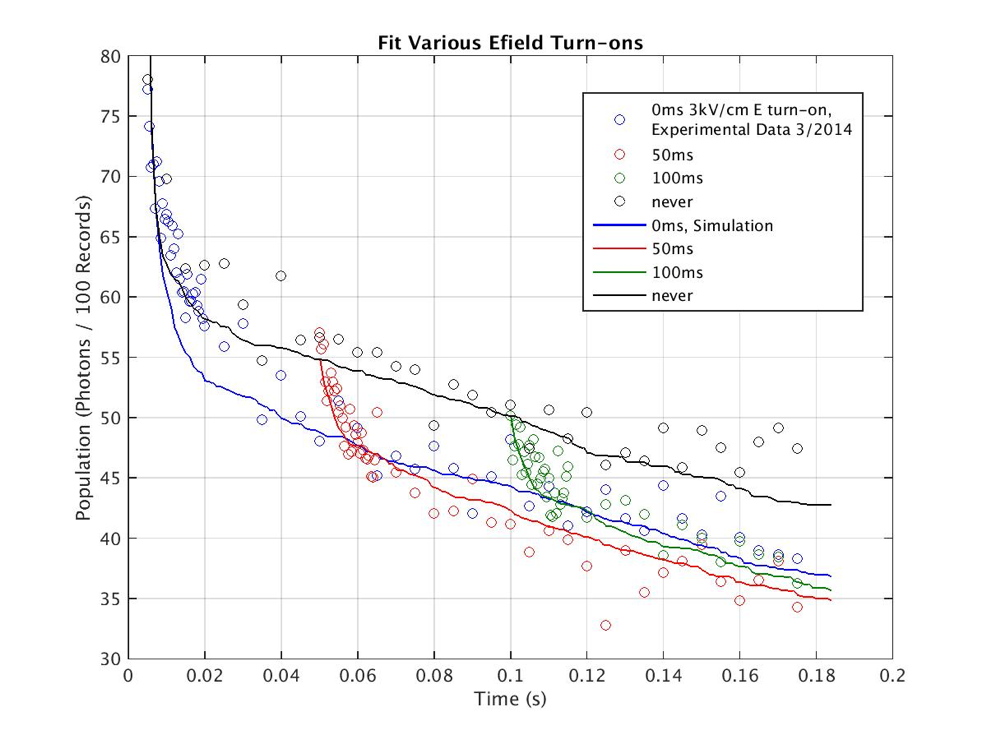
\includegraphics[width=4cm]{SuppFigs/EIL.png}%
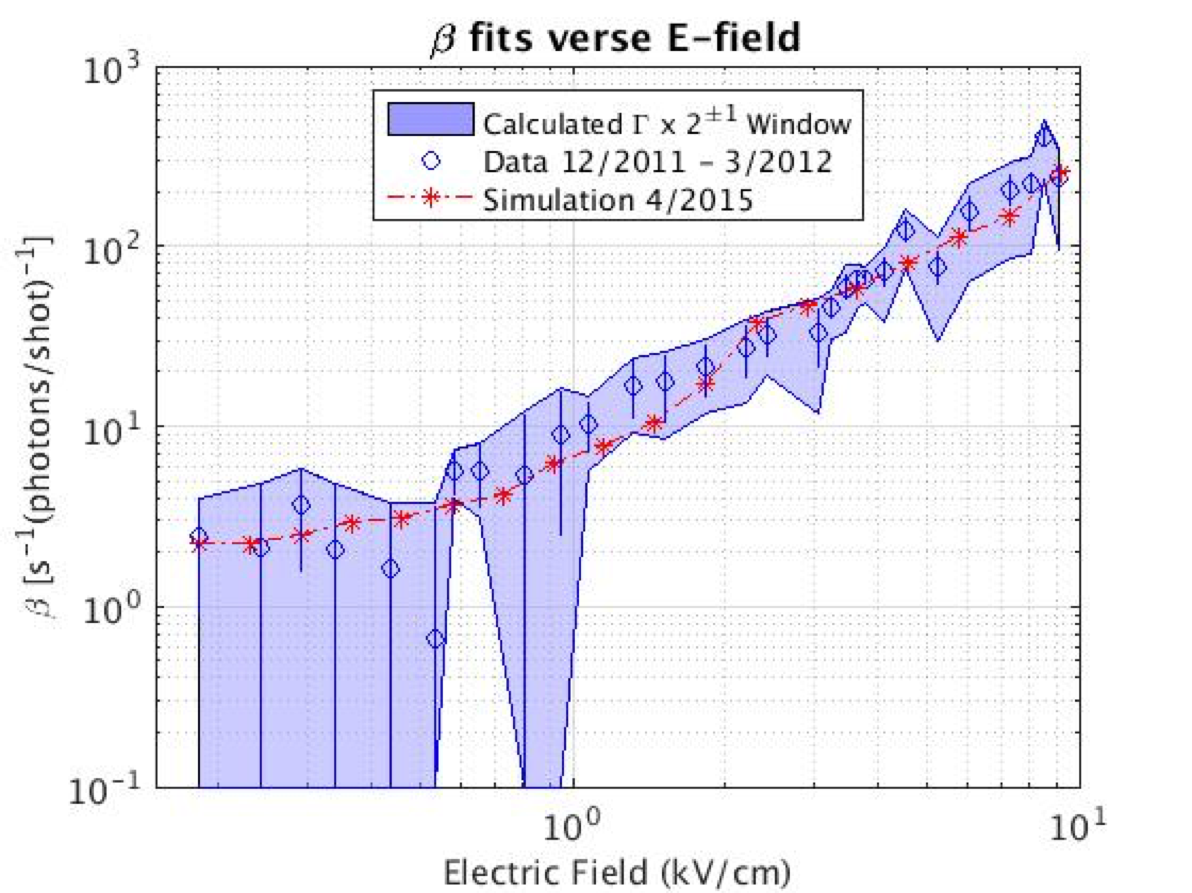
\includegraphics[width=4cm]{SuppFigs/Beta.png}%
\caption{
(a) Experimental E-field induced loss data with an attempted overlap to spin-flip loss simulations. (b) Two body fits from~\cite{Stuhl2013} with overlapped spin flip loss single particle simulation in red stars.
}
\label{fig:eil}
\end{figure}

We can perform purely single particle simulations of spin-flip loss to investigate this, and we obtain curves such as shown above the time dependent experiment data points in fig.~\ref{fig:eil}(a).
The simulations do predict a loss rate that turns off over time, and they do a decent job matching the magnitude of the loss induced by the electric field.
We can even perform a two body fitting procedure like the one used in~\cite{Stuhl2013} to the data obtained from this single particle spin-flip loss simulation, see fig.~\ref{fig:eil}(b). 
This suggests that the effect attributed to two-body collisions could be largely explained by spin-flip losses.
Of course there are notable differences, such as in the initial rate of decay in fig.~\ref{fig:eil}(a) 
One avenue to try and be more quantitative would be to incorporate collisions in the simulation and see what collision rates yield the best agreement between simulation and experiment.
Unfortunately there are many challenges in the quantitative application of simulations such as these, such as uncertainty regarding the initial distribution and the existence of various partially trapped substates.
We think the best path forward is to perform future collisional studies with the single-particle effect removed, as described in the main text.

With regard to~\cite{Stuhl2012evap}, the present study is only one of a number of important modifications to our understanding that have come up in the past few years. 
The first is related to the approximate Hamiltonian used for interpretation of microwave spectroscopies. 
As discussed in~\cite{Maeda2015}, where a thorough investigation of hyperfine shifts and external field effects is performed for OH, this approximate Hamiltonian requires a $15\%$ correction to the magnetic dipole moment, and thus to the magnetic field at a particular microwave frequency. 
This would only shift the fitted temperatures slightly colder, except that it also changes the location of avoided crossings, and renders the assumption of a Boltzmann suppression factor related to these crossings untenable.
This suppression factor was related to the mechanics of the spectroscopy performed in~\cite{Stuhl2012evap}, which ought to be insensitive to molecules below the lowest avoided crossing.
The data show a sudden suppression below $480\text{ G}$, but the crossing is actually located closer to $400\text{ G}$.
Without this, the fits used to calculate temperature when the population ought to be significantly built-up at lower magnetic fields are no longer trustworthy. 

In fact, the unreliability of the deeper cutting spectra in~\cite{Stuhl2012evap} is the same conclusion implied by the present study of spin-flip losses.
At the temperatures fitted to those spectra, the spin-flip loss caused by the E-field used during evaporation are large enough to significantly influence the population, see the table in the main text.
Nonetheless, even after abandoning the inferred population build-up at lower fields, it is still possible to use normalized spectra to look for any enhancements in density caused by the evaporation procedure.
For the shallowest cut in~\cite{Sthul2012evap}, normalized spectra comparison show a nice pileup beginning near $500\text{ G}$, compare the red and black traces in fig.~\ref{fig:normenhance}.
The normalization is simply a rescaling of the traces in order to match the area under the distribution to the total molecule number measured directly by laser induced fluorescence.

\begin{figure}[tb]
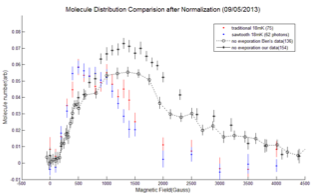
\includegraphics[width=\linewidth]{SuppFigs/NormEnhance.png}%
\caption{
Normalized spectra show a clear increase in molecule density near $500\,\text{G}$.
}
\label{fig:normenhance}
\end{figure}

We have also developed a few more sensitive tools to look for collisional or evaporative effects, in addition to the microwave depletion during deceleration described and used in the main text.
One is to compare the populations under two related conditions- the first a normal evaporation sequence and the second an evaporation with time-reversed microwave frequency. 
In other words, the cut goes backwards from deep to shallow. 
This comparison subjects all molecules to the same integrated microwave power, and thus the two conditions would be equivalent in a situation with only single particle effects. 
With evaporative effects, the normal condition ought to perform better. 
This is indeed what we consistently observe, at the 5\% level, see fig.~\ref{fig:normenhance}.

We have also pursued the precise calibration of our LIF system, using a careful comparison to Raman scattering of $\text{H}_2$, as described in~\cite{Bischel1986}. 
Our results suggest that since 2014, our molecule number has been about $1000$, yielding a peak density of $10^7/\text{cm}^3$ assuming a thermal distribution, and a collision rate of not more than $0.1/\text{s}$.
At this rate, only $1\%$ of molecules collide during a $100\text{ ms}$ experiment, and only a fraction of those collisions would result in cooling. 
Nonetheless, there are uncertainties with the calibration, and it is possible that some decline in system performance could be involved, since we have a record of decreased voltage conditioning performance in our decelerator.

In conclusion, the collisional results in~\cite{Stuhl2012evap,Stuhl2013} are significantly weakened by spin-flip losses and other modifications to our understanding. The density may simply have been too low, although back-application to the 2012-13 systems used is not perfect. Spectroscopic comparisons and evaporation subtractions do suggest a slight evaporative effect, and the development of various more sensitive tools has us poised to more unambiguously identify any future collisional effects in our next generation system described in the main text.

%includes uncited bib entries
%\nocite{*}
\bibliographystyle{apsrev4-1_no_Arxiv}
\bibliography{Supplement}

\end{document}
%
% ****** End of file MolecularMajoranaLoss.tex ******
